\section{The Wolfram Hypergraph Sieve (Phase 2)}

While Phase 1 relies on stochastic optimization, Phase 2 seeks a deterministic origin for the compactification geometry using discrete pre-geometry inspired by the Wolfram Physics Project.

We define a vacuum hypergraph seeded by a $K_4$ complete graph embedded within an 11-node ring. The adjacency matrix $M$ of this structure has dimension $15 \times 15$. The topological properties of this network are extracted via the trace of its powers, yielding the causal loop sequence:
\begin{equation}
    W(n) = \mathrm{Tr}(M^n)
\end{equation}

\subsection{Spectral Radius and Apéry Sequences}
The exact decomposition of this sequence is dominated by the pure $K_4$ component:
\begin{equation}
    W_{K_4}(n) = \frac{3^n + 3(-1)^n}{4}
\end{equation}
This directly corresponds to OEIS A054878 (Number of closed walks on a $K_4$ graph). The dominant eigenvalue (spectral radius) is exactly $\lambda_1 = 3.0$.

In algebraic geometry, the spectral radius of the Picard-Fuchs differential operator dictates the complex structure moduli space. A spectral radius of 3.0 uniquely isolates the Cooper $s_{10}$ sequence (OEIS A291898), terminating the search space deterministically.

\begin{figure}[h]
    \centering
    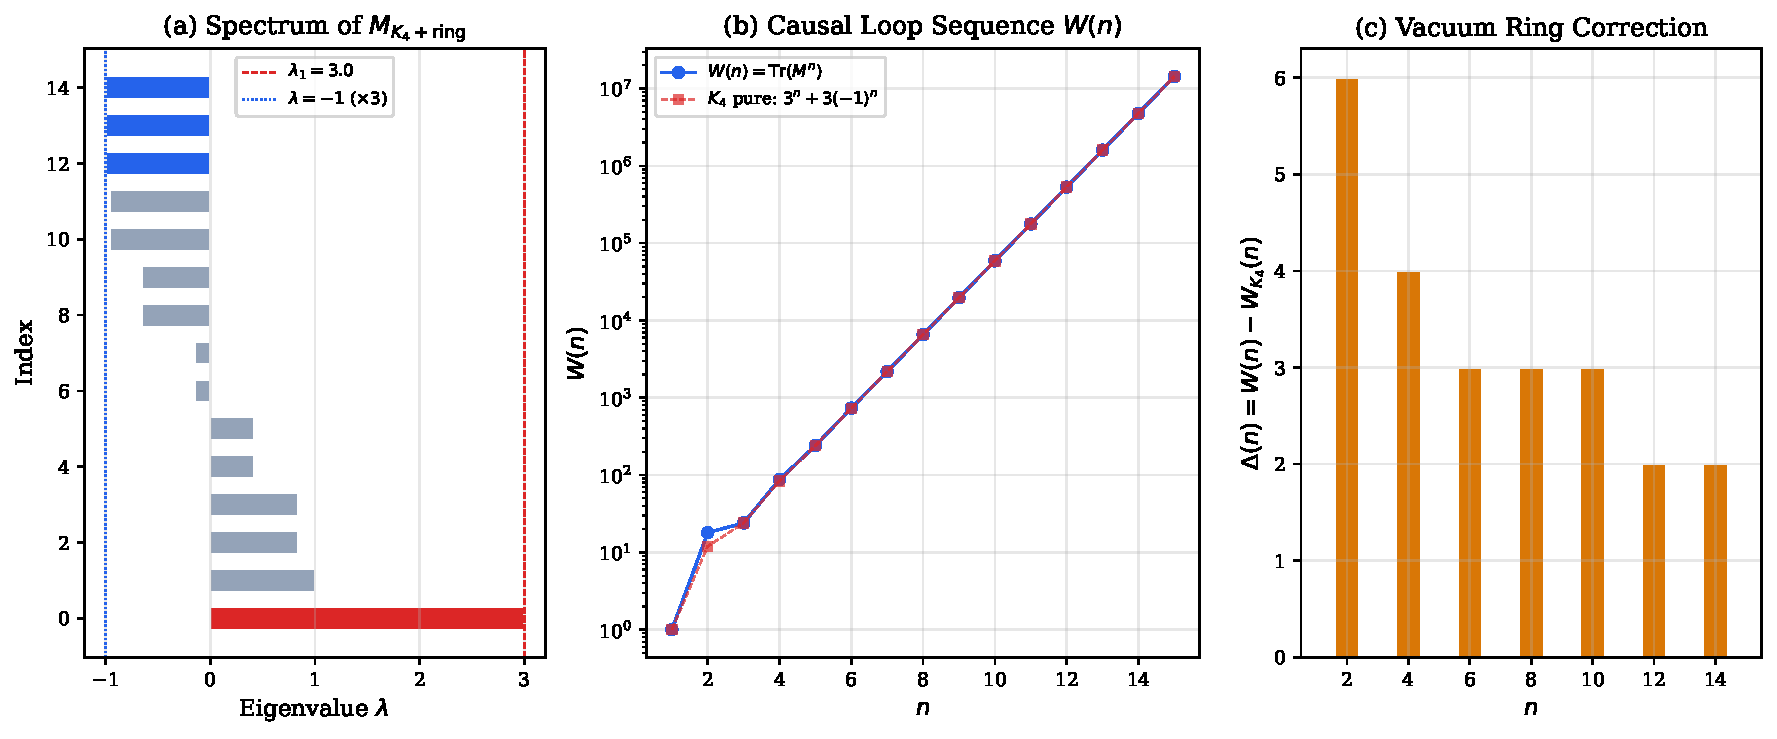
\includegraphics[width=\textwidth]{figures/spectral_sieve.pdf}
    \caption{Spectral Sieve mapping $K_4$ eigenvalues to the $W(n)$ causal loop sequence.}
\end{figure}
